\documentclass{article}
\usepackage{graphicx,float}
\usepackage{amsmath,latexsym,amsfonts,amssymb,amsthm}

\usepackage[utf8]{inputenc}
\usepackage[english]{babel}
\usepackage[letterpaper,top=2cm,bottom=2cm,left=3cm,right=3cm,marginparwidth=1.75cm]{geometry}
\renewcommand{\baselinestretch}{1.667}


\title{Optimization Methods PS s7 Lab 4}
\author{Joris Plaščinskas}
\date{\today}


\begin{document}


\maketitle
\section*{Linear Simplex Algorithm}
Linear simplex algorithm is an iterative optimization method used to find the optimal values of a linear problem (all constraint and objective function are linear). The algorithm generally follows these steps:
\begin{itemize}
    \item \textbf{Formalize the problem into standard form}. The problem is given in inequalities form. The standard form uses equations, so the inequalities will have to be rewritten. We do this by adding slack variables, each constraint will get it's own $s_i$ variable that represents how far away from being strict it is. If the slack variable is 0, that means the constraint is tight.
    \item \textbf{Initialize tableau}. In the middle are the constraint coefficients, on the right are RHS values. Bottom row is objective function coefficients. And the bottom right cell is objective function value. An example table can be seen below:
    \begin{figure}[H]
        \centering
        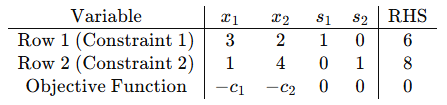
\includegraphics[width=0.333\textwidth]{tableau-example.png}
        \caption{Tableau Example}
        \label{fig:tableau-example}
    \end{figure}
    \item \textbf{While optimal value is not reached, iterate on the below steps}. Optimal value is reached when all of the values in the objective function row in tableau are negative, that means there is no way to increase it more (for maximization problems).
    \begin{itemize}
        \item \textbf{Identify the entering variable}. The entering variable is selected by looking at the bottom (objective) row and selecting the highest negative value.
        \item \textbf{Identify the leaving variable}. For each row calculate the ratio of RHS of the constraint to the coefficient of the entering variable in that row. Only consider rows where the coeeficient of the entering variable is positive
        \item \textbf{Perform a pivot around the pivot variable}. First we need to divide the pivot row by the pivot element to make the pivot element equal to 1. Then we adjust the other rows to make all other elements in the pivot column equal to 0.
    \end{itemize}
\end{itemize}
The code can be seen in the image below:
\begin{figure}[H]
    \centering
    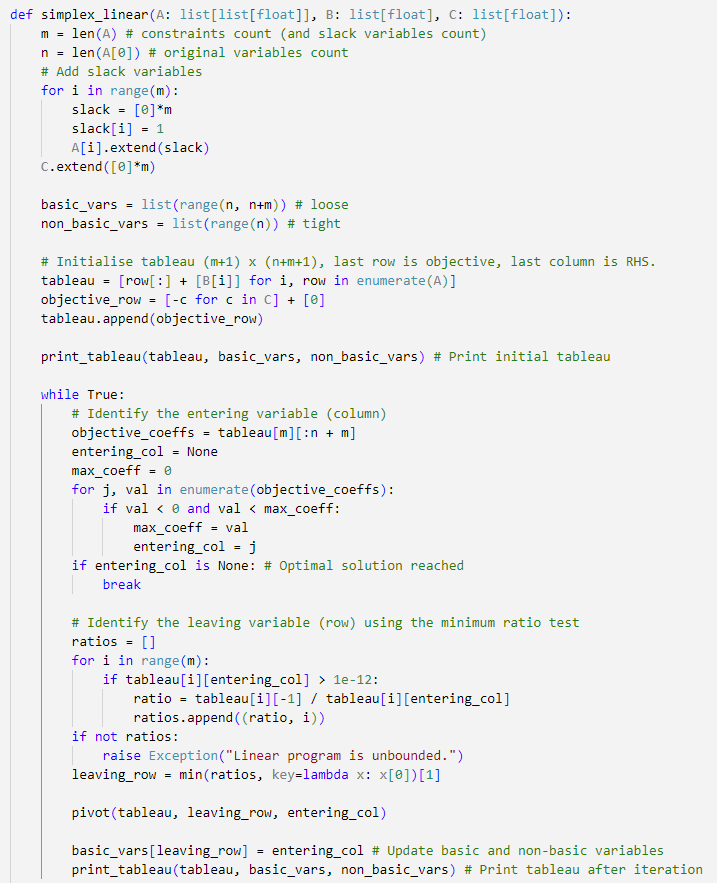
\includegraphics[width=1\textwidth]{simplex-linear.png}
    \caption{Simplex Implementation}
    \label{fig:simplex-implementation}
\end{figure}

\section*{Exercise in Matrix Form}
\[
\begin{aligned}
\text{Maximize} \quad & \mathbf{c}^\top \mathbf{x} \\
\text{where} \quad & \mathbf{c} = 
\begin{bmatrix}
-2 \\
\,\,3 \\
\,\,0 \\
\,\,5 \\
\,\,0 \\
\,\,0 \\
\,\,0 
\end{bmatrix}, \\
\text{subject to} \quad & \mathbf{A} \mathbf{x} = \mathbf{b}, \\
& \mathbf{A} =
\begin{bmatrix}
-1 & 1 & -1 & -1 & 1 & 0 & 0 \\
\,\,2 & 4 & \,\,0 & \,\,0 & 0 & 1 & 0 \\
\,\,0 & 0 & \,\,1 & \,\,1 & 0 & 0 & 1 
\end{bmatrix}, \quad
\mathbf{b} =
\begin{bmatrix}
8 \\
10 \\
3 
\end{bmatrix}, \\
& \mathbf{x} \geq \mathbf{0}
\end{aligned}
\]

\section*{Results and Conclusion}
\begin{figure}[H]
    \centering
    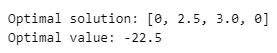
\includegraphics[width=0.5\textwidth]{solution-standard.png}
    \caption{Solution Standard}
    \label{fig:simplex-implementation}
\end{figure}
\begin{figure}[H]
    \centering
    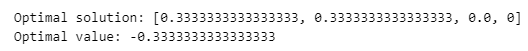
\includegraphics[width=0.5\textwidth]{solution-my.png}
    \caption{Solution My}
    \label{fig:simplex-implementation}
\end{figure}
Both in the standard exercise solution and in my version, the second and third constraints are active, which means they have the same base.

\end{document}